\documentclass{article}

\usepackage[hyphens]{url}
\usepackage[hidelinks]{hyperref}

\usepackage[utf8]{inputenc}
\usepackage[T1]{fontenc}
\usepackage[british,swedish]{babel}

\usepackage{noweb}
\usepackage{booktabs}

\usepackage[natbib,style=alphabetic,maxbibnames=99]{biblatex}
\addbibresource{bibliography.bib}

\usepackage[all]{foreign}
\renewcommand{\foreignfullfont}{}
\renewcommand{\foreignabbrfont}{}

%\usepackage{newclude}
\usepackage{import}

\usepackage[strict]{csquotes}
\usepackage[single]{acro}

\usepackage{subcaption}

\usepackage[noend]{algpseudocode}
\usepackage{xparse}

\let\email\texttt

\usepackage[outputdir=ltxobj]{minted}
\setminted{autogobble,linenos}

\usepackage{pythontex}
\setpythontexoutputdir{.}
\setpythontexworkingdir{..}

\usepackage{amsmath}
\usepackage{amssymb}
\usepackage{mathtools}
\usepackage{amsthm}
\usepackage{thmtools}
\usepackage[unq]{unique}
\DeclareMathOperator{\powerset}{\mathcal{P}}

\usepackage[binary-units]{siunitx}

\usepackage{hyperref}
\usepackage[swedish]{cleveref}


\usepackage[noamsthm,notheorems]{beamerarticle}
\setjobnamebeamerversion{slides}

%\usepackage{authblk}
%\let\institute\affil

\declaretheorem[numbered=unless unique,style=theorem]{theorem}
\declaretheorem[numbered=unless unique,style=definition]{definition}
\declaretheorem[numbered=unless unique,style=definition]{assumption}
\declaretheorem[numbered=unless unique,style=definition]{protocol}
\declaretheorem[numbered=unless unique,style=example]{example}
%\declaretheorem[style=definition,numbered=unless unique,
%  name=Example,refname={example,examples}]{example}
\declaretheorem[numbered=unless unique,style=remark]{remark}
\declaretheorem[numbered=unless unique,style=remark]{idea}
\declaretheorem[numbered=unless unique,style=exercise]{exercise}
\declaretheorem[numbered=unless unique,style=exercise]{question}
\declaretheorem[numbered=unless unique,style=solution]{solution}

\begin{document}
\title{%
  En väg genom studierna
}
\author{Daniel Bosk}
\institute{%
  KTH EECS
}

\maketitle

\begin{abstract}
  % What's the problem?
% Why is it a problem? Research gap left by other approaches?
% Why is it important? Why care?
% What's the approach? How to solve the problem?
% What's the findings? How was it evaluated, what are the results, limitations, 
% what remains to be done?

I den här modulen skriver vi ett program som låter användaren kryptera och 
avkryptera meddelanden.
Syftet är att illustrera enkla algoritmiska problem och alla grundläggande 
programmeringstekniska konstruktioner; såsom funktioner och kontrollflöden.
Syftet är också att inspirera till reflektion om säkerhet och kryptografi.

\emph{Lärandemål:}
Efter att ha genomfört modulen ska den lärande kunna:
\begin{itemize}
  \item läsa grundläggande programkod med enkla konstruktioner
    och, mestadels korrekt, förklara vad koden gör;
  \item konstruera enkla algoritmer (inte syntaktiskt korrekt programkod) på en 
    detaljnivå lämpad för programmering, exempelvis att man måste läsa bokstav 
    för bokstav och göra någonting för varje.
  \item förklara vad kryptering och avkryptering är och varför det är viktigt.
\end{itemize}

\end{abstract}

\mode*

\begin{frame}
  \tableofcontents
\end{frame}

% Vad har matte med programmering att göra? KORT (=enstaka minut)
% 
% Vad är kryptering? Kanske en 10 minutersuppgift där klassen ska kryptera 
% ordet "pannkaka" på valfritt sätt och sedan ett resonemang kring vad som är 
% säker och osäker kryptering.
% 
% Ett program för att testa säkerheten i ett lösenord, för "lek" timmen efter.

\section{Programmering?}

% Fokus programmering (=vad är programmering), varför läsa programmering, 
% datasäkerhet/kryptering. Bra att få med:

\begin{frame}
  \begin{question}
    \begin{itemize}
      \item Vad är programmering?
      \item Var finns programmering?
      \item Vad är det bra för?
      \item Hur kan programmering vara farligt?
    \end{itemize}
  \end{question}
\end{frame}

\subsection{Vad är programmering?}

\begin{frame}
  \begin{block}{Vad är programmering?}
    \begin{itemize}
      \item Programmering betyder att skriva program.
      \item Program implementerar algoritmer, exempelvis gör så att datorn kan 
        köra en viss algoritm.
      \item Algoritmer är sätt att göra någonting på.
    \end{itemize}
  \end{block}

  \pause

  \begin{exercise}[Välkända algoritmer]
    \begin{itemize}
      \item Känner ni till några algoritmer?
    \end{itemize}
  \end{exercise}
\end{frame}

\begin{frame}
  \begin{example}[Att göra pannkakssmet]
    \begin{enumerate}
      \item Knäck tre ägg i en bunke.
      \item Vispa ordentligt.
      \item Häll i \SI{3}{\deci\litre} mjölk.
      \item Vispa ordentligt.
      \item För totalt \SI{3}{\deci\litre} mjöl:
        \begin{enumerate}
          \item Häll i \SI{1}{\deci\litre} mjöl.
          \item Vispa ordentligt.
        \end{enumerate}
      \item Häll i \SI{\frac{1}{2}}{tsk} salt.
      \item Häll i \SI{2}{msk} smält smör.
      \item Vispa ordentligt.
    \end{enumerate}
  \end{example}
\end{frame}

\begin{frame}
  \begin{example}[Att steka pannkakor]
    \begin{enumerate}
      \item Gör pannkakssmet.
      \item För varje portion:
        \begin{enumerate}
          \item Häll \SI{1}{\deci\litre} smet i en het stekpanna.
          \item Vänta \SI{2}{\minute}.
          \item Vänd pannkakan.
          \item Vänta \SI{2}{\minute}.
          \item Servera pannkakan.
        \end{enumerate}
    \end{enumerate}
  \end{example}
\end{frame}

%\begin{frame}
%  \begin{example}[Knyta skorna, en variant]
%    \begin{enumerate}
%      \item Korsa snörena.
%      \item Låt den ena gå igenom öglan.
%      \item Dra åt.
%      \item Gör den ena till en ögla.
%      \item Gör den andra till en ögna.
%      \item Korsa dem.
%      \item Låt den ena gå igenom öglan.
%      \item Dra åt.
%    \end{enumerate}
%  \end{example}
%\end{frame}

\begin{frame}
  \begin{remark}
    \begin{itemize}
      \item Kokbok: en samling program för köket.
      \item Exekveras inte av datorer.
      \item Det är människor som exekverar dem.
    \end{itemize}
  \end{remark}

  \pause

  \begin{remark}
    \begin{itemize}
      \item Datorprogram implementerar algoritmer som kan exekveras av datorer.
    \end{itemize}
  \end{remark}
\end{frame}


\subsection{Var finns programmering?}

% Var finns programmering?

\begin{frame}
  \begin{exercise}
    \begin{itemize}
      \item Var finns programmering?
    \end{itemize}
  \end{exercise}
\end{frame}

\begin{frame}
  \begin{example}[Fordon]
    \begin{itemize}
      \item Sitter hundratals datorer i en bil idag.
    \end{itemize}
  \end{example}

  \begin{example}[Ekonomiska system]
    \begin{itemize}
      \item Bankomaterna
      \item Internetbanken
      \item Swish
      \item Terminalerna i butikerna
    \end{itemize}
  \end{example}

  \begin{example}[Kritisk infrastruktur]
    \begin{itemize}
      \item Kraftverk
      \item Industriell produktion
    \end{itemize}
  \end{example}
\end{frame}

\begin{frame}
  \begin{example}[Servrar på webben]
    \begin{itemize}
      \item Varenda webbsida är utmatningen av ett program.
      \item Ibland innehåller själva webbsidan program som webbläsaren kör 
        (Javascript).
    \end{itemize}
  \end{example}
\end{frame}

\subsection{Vad är det bra för?}

\begin{frame}
  \begin{question}
    \begin{itemize}
      \item Varför göra något som en dator/robot kan göra bättre?
    \end{itemize}
  \end{question}
\end{frame}

\begin{frame}
  \begin{example}[Hemautomation]
    \begin{itemize}
      \item Robotdammsugare
      \item Robotgolvmoppar
      \item Automatiska lysen (var någon är hemma, om solen gått ned)
      \item Kontroll av energianvändning
    \end{itemize}
  \end{example}
\end{frame}

\begin{frame}
  \begin{example}[Automation i mitt jobb]
    \begin{itemize}
      \item Föra över betyg från lärplattformen till nationella 
        betygsdatabasen.
      \item Samla in statistik för hur det går för studenterna.
    \end{itemize}
  \end{example}

  \begin{example}[Räkna på data]
    \begin{itemize}
      \item Vad är Sveriges vanligast namn?
      \item Får eleverna högre betyg i matematik efter att de lärt sig att 
        programmera?
    \end{itemize}
  \end{example}
\end{frame}

% Ett program kan endast utföra de operationer som tilldelats, det tänker inte 
% själv.

\begin{frame}
  \begin{example}[\enquote{Framtida} automation]
    \begin{itemize}
      \item Självkörande fordon
      \item \enquote{Smarta} städer
    \end{itemize}
  \end{example}

  \pause

  \begin{remark}
    \begin{itemize}
      \item Datorer är inte smartare än vad vi gör dem.
      \item De följer bara instruktioner.
    \end{itemize}
  \end{remark}
\end{frame}


\section{Hur kan detta vara farligt?}

% Hur kan programmering användas på ett skadligt sätt?

% Programkoden är (i ett normalt interface) osynlig för användaren, användaren 
% vet inte vad programmet gör i bakgrunden.

% Användaren vet inte vilken information som insamlas/används. Exempel: 
% Facebook följer allt du gör på nätet, t.ex. hur du surfar mellan hemsidor och 
% vilka. Detta sker även när du inte är inloggad.

% Många program (s.k. bottar) är framtagna för att bedriva propaganda, påverka 
% val och manipulera resultat/statistik. Dessa program analyserar användaren 
% och tar reda på hur du tänker tycker i dagsläget, för att så effektivt som 
% möjligt påverka dig att tycka och tänka annorlunda.

\begin{frame}
  \begin{figure}
    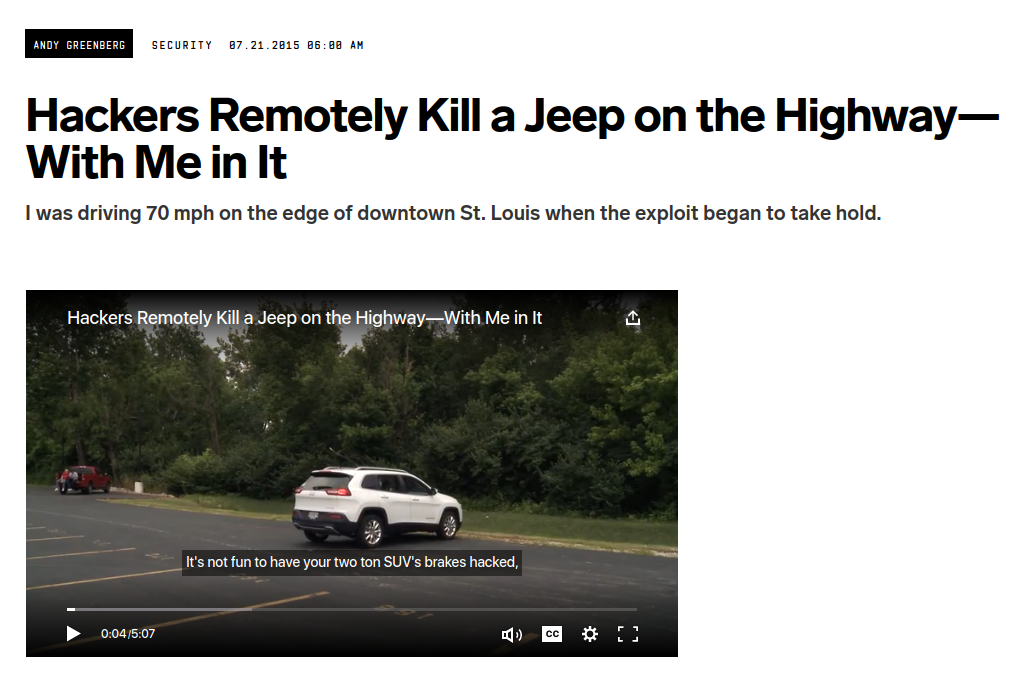
\includegraphics[width=\columnwidth]{fig/hacking-jeep.png}
  \end{figure}
\end{frame}

\begin{frame}
  \begin{example}[Spårning på webben]
    \begin{itemize}
      \item \url{https://clickclickclick.click}
      \item \url{https://amiunique.org/}
      \item \url{https://coveryourtracks.eff.org/}
    \end{itemize}
  \end{example}
\end{frame}

\begin{frame}
  \begin{question}
    \begin{itemize}
      \item Fine, de kan spåra mig på webben.
      \item Varför bry sig?
    \end{itemize}
  \end{question}
\end{frame}

\begin{frame}
  \begin{figure}
    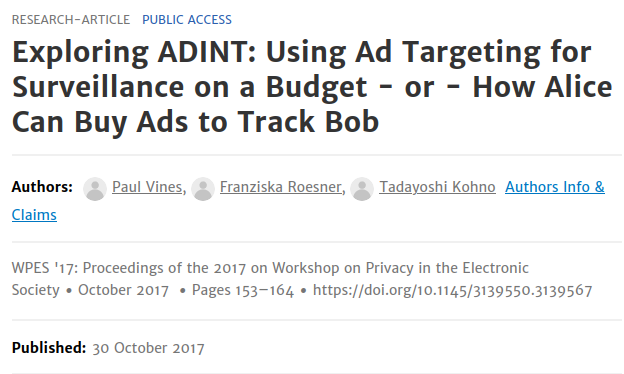
\includegraphics[width=\columnwidth]{fig/adint.png}
  \end{figure}
\end{frame}

\begin{frame}
  \begin{figure}
    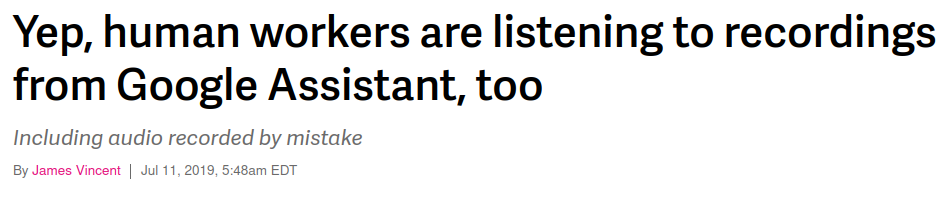
\includegraphics[width=\columnwidth]{fig/listening-assistants.png}
  \end{figure}
\end{frame}

\begin{frame}
  \begin{figure}
    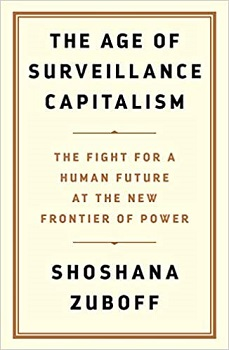
\includegraphics[height=0.8\textheight]{fig/The-Age-of-Surveillance-Capitalism.jpg}
  \end{figure}
\end{frame}

\begin{frame}
  \begin{figure}
    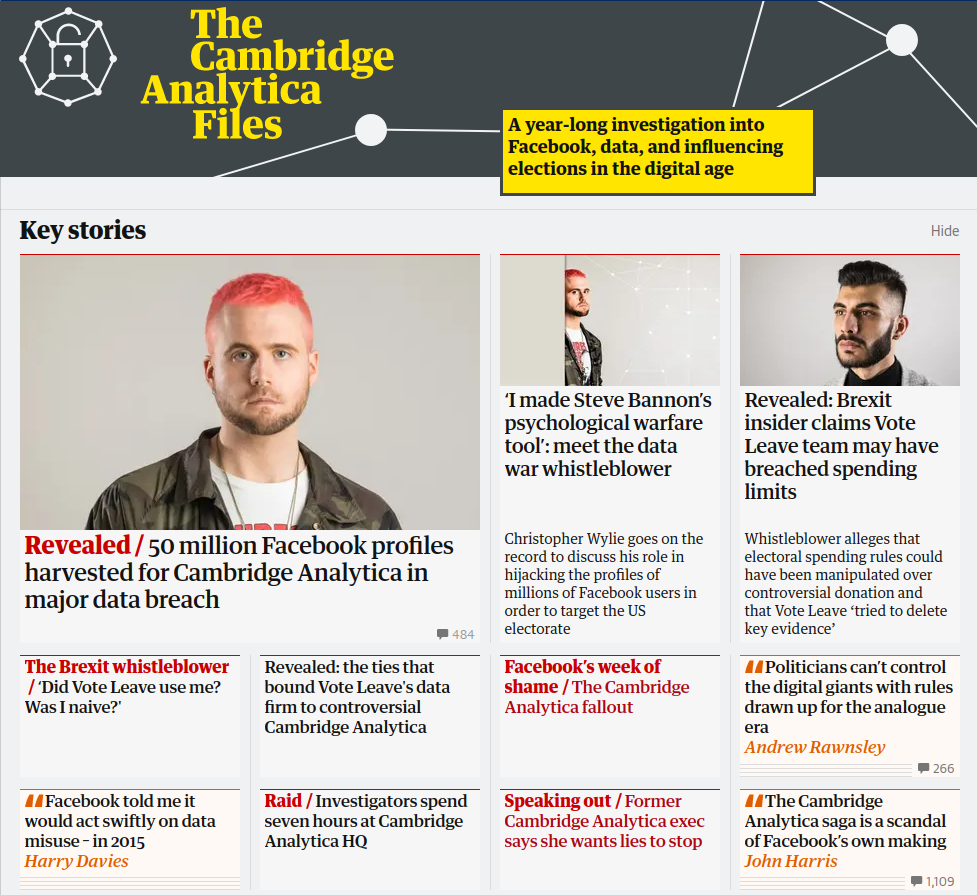
\includegraphics[width=\columnwidth]{fig/analytica.png}
  \end{figure}
\end{frame}

\begin{frame}
  \begin{figure}
    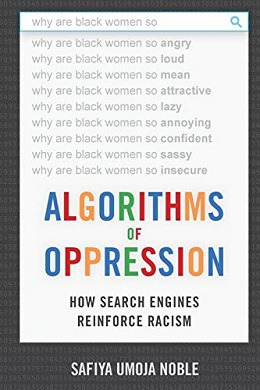
\includegraphics[height=0.8\textheight]{fig/Algorithms-of-Oppression.jpg}
    \only<2>{%
      
\includegraphics[width=0.6\columnwidth]{fig/teens.png}
    }
  \end{figure}
\end{frame}

\begin{frame}
  \begin{figure}
    
\includegraphics[height=0.8\textheight]{fig/Automating-Inequality.jpg}
    \hspace{2em}
    
\includegraphics[height=0.8\textheight]{fig/Weapons-of-Math-Destruction.jpg}
  \end{figure}
\end{frame}

\begin{frame}
  \begin{question}
    \begin{itemize}
      \item Hur många var det som tänkte på att alla dessa böcker var skrivna 
        av kvinnor?
    \end{itemize}
  \end{question}
\end{frame}

%\begin{frame}
%  \begin{remark}
%    \begin{itemize}
%      \item Finns massor med problem med saker som automatiserad 
%        beslutsfattning.
%      \item Rekommendationsalgoritmer skapar filterbubblor.
%      \item Och mycket mer.
%    \end{itemize}
%  \end{remark}
%\end{frame}

% Många appar innehåller malware (sabotageprogram) som t.ex. stjäl användarens 
% bilder för att skicka/sälja vidare till tredje part eller ''lyssnar'' på vad 
% du säger genom mikrofonen, även när du är inaktiv.

% Våra samhällssystem bygger på kod och har svagheter (särskilt när någon går 
% in med avsikt att skada system eller läcka information) och därmed föreligger 
% förstås både mindre och större risker, från att mailkonton hackas till att 
% elnät släcks ned.

% Alla system måste byggas med rigida skydd mot sabotage.
% Förhoppningsvis ska detta inte avskräcka utan intressera för vad som
% är och kommer att fortsätta vara ett enormt utvecklingsområde.
% Lektion 8 handlar om arbetsmöjligheter inom data, informationsteknologi (IT), 
% programmering osv. Där kryptering (omkodning av data för att t.ex. skydda 
% lösenord och öka vår personliga säkerhet online) är ett enormt och växande 
% område.

% Dina tankar om GDPR: tillräcklig förordning? Gäller för EU:s
% medborgare, men även amerikanska företeg( tex facebook) måste väl
% tillse att det följs för europeiska användare? Har USA motsvarande
% (bättre/sämre) personuppgiftslag\ldots{}?

% En tanke jag har är att eleverna tror att GDPR skyddar dem\ldots{} men
% så fort de klickar ``godkänn cookies'' så har dom delgivit till saker
% som dom inte har en aning om\ldots{} Inte ens jag vet vad man godkänner,
% ändå klickar man ``godkänn alla'' typ överallt för att komma
% vidare\ldots{} Vad ger man då bort liksom\ldots{}? Det är dom nyfikna
% på.

%\begin{frame}
%  \begin{figure}
%    
\includegraphics[height=\textheight]{fig/tay.ai.png}
%  \end{figure}
%\end{frame}

% Varför kul/bra att utbilda sig inom och jobba med programmering? (mycket 
% samarbete kanske... bra lön, ökande efterfrågan på kompetens på området)

\section{Varför programmering?}

\begin{frame}
  \begin{example}[Förståelse]
    \begin{itemize}
      \item Nästintill allt är programmerat.
      \item Man behöver ha en förståelse för programmering för att förstå 
        världen.
    \end{itemize}
  \end{example}

  \begin{example}[Arbete]
    \begin{itemize}
      \item Fler arbeten kommer att kunna automatiseras med programmering.
      \item Kommer att behövas många fler som kan programmera.
    \end{itemize}
  \end{example}
\end{frame}

\section{Vad är matematik?}

% Eleverna ska tycka att programmering är intressant och förstå att 
% mattekunskaper är bra att ha :D

\begin{frame}
  \begin{example}<1,3>
    \begin{itemize}
      \item En triangel har basen \SI{\alert<3>2}{\centi\metre} och höjden 
        \SI{\alert<3>3}{\centi\metre}.
      \item En rektangel har basen \SI{\alert<3>2}{\centi\metre} och höjden 
        \SI{\alert<3>3}{\centi\metre}.
      \item Hur mycket större area har rektangeln?
    \end{itemize}
  \end{example}

  \begin{example}<2,3>
    \begin{itemize}
      \item En triangel har basen \(\SI{\alert<3>b}{\centi\metre}\) och höjden 
        \(\SI{\alert<3>h}{\centi\metre}\).
      \item En rektangel har basen \(\SI{\alert<3>b}{\centi\metre}\) och höjden 
        \(\SI{\alert<3>h}{\centi\metre}\).
      \item Kommer rektangeln alltid att ha dubbla arean?
    \end{itemize}
  \end{example}
\end{frame}

\begin{frame}
  \begin{solution}
    \begin{itemize}
      \item Ja, rektangeln kommer alltid att ha dubbla arean.
      \item Arean för rektangeln är \(bh\), medan arean för triangeln är 
        \(\frac{1}{2}bh\).
      \item \(b\) och \(h\) var ju desamma i båda fallen.
    \end{itemize}
  \end{solution}
\end{frame}

\subsection{Varför är det centralt för datasäkerhet?}

\begin{frame}
  \begin{remark}
    \begin{itemize}
      \item Vi kan inte testa säkerheten.
      \item Vi vet inte hur angriparen kommer att göra.
      \item Vi måste veta att hur angriparen än gör, så lyckas hen inte.
    \end{itemize}
  \end{remark}

  \pause

  \begin{example}
    \begin{itemize}
      \item Att testa säkerheten är som att testa att rektangeln har mer area 
        än triangeln.
    \end{itemize}
  \end{example}
\end{frame}

\begin{frame}
  \begin{solution}
    \begin{itemize}
      \item Vi behöver arbeta systematiskt och deduktivt med matematik.
    \end{itemize}
  \end{solution}
\end{frame}

\begin{frame}
  \begin{exercise}
    \begin{itemize}
      \item Anna valde sitt lösenord på följande sätt:
      \item Hon valde ett ord hon tycker om, sedan lade hon till två siffror 
        och ett specialtecken i slutet.
      \item En dator kan gissa mellan 100\,000 och 1\,000\,000 lösenord per 
        sekund.
      \item Hur lång tid tar det att knäcka Annas lösenord?
    \end{itemize}
  \end{exercise}

  \pause

  \begin{exercise}
    \begin{itemize}
      \item Lars valde sitt lösenord annorlunda.
      \item Han valde ett ord och översatte det till 1337-speak.
      \item Hur lång tid tar det att knäcka hans lösenord?
    \end{itemize}
  \end{exercise}
\end{frame}

\begin{frame}
  \begin{solution}
    \begin{itemize}
      \item<+-> Hur många ord har de att välja mellan?
      \item<+-> Svenska Akademiens Ordlista har ungefär 125\,000 ord: 
        \(125\,000^1\) möjligheter.
      \item<+-> Anna valde två siffror och ett specialtecken slumpmässigt: 
        \(10^3\) möjligheter.
      \item<+-> Lars ändrade till 1337-speak, detta är deterministiskt: \(1\) 
        möjlighet.
      \item<+-> Den \alert{långsamma} datorn behöver \(\frac{125\,000\cdot 
        10^3}{100\,000} = 1250\) sekunder, eller strax under 21 minuter för att 
        knäcka Annas lösenord.
      \item<+-> Den \alert{långsamma} datorn behöver \(\frac{125\,000\cdot 
        1}{100\,000} = 
        1.25\) sekunder för Lars lösenord.
    \end{itemize}
  \end{solution}
\end{frame}

\begin{frame}
  \begin{exercise}
    \begin{itemize}
      \item Evin valde fyra slumpmässigt valda ord ur Svenska Akademiens 
        Ordlista som sitt lösenord.
      \item Inga siffror, inga specialtecken, inget 1337-speak.
      \item Hur lång tid tar det att knäcka hennes lösenord?
    \end{itemize}
  \end{exercise}
\end{frame}

\begin{frame}
  \begin{solution}
    \begin{itemize}
      \item Evin valde fyra slumpmässiga ord: det ger \(125\,000^3\) 
        möjligheter.
      \item Den \alert{snabba} datorn behöver \(\frac{125\,000^3}{1\,000\,000} 
        = 1953125000\) sekunder, eller 62 år.
    \end{itemize}
  \end{solution}
\end{frame}

\begin{frame}
  \begin{question}
    \begin{itemize}
      \item Kommer Evins sätt att välja lösenord alltid att vara bättre?
      \item Finns det bättre gissningsalgoritmer som knäcker hennes lösenord 
        snabbare?
    \end{itemize}
  \end{question}
\end{frame}

\begin{frame}
  \begin{question}
    \begin{itemize}
      \item Egentligen borde det ta hälfen så lång tid i medel.
      \item Varför?
    \end{itemize}
  \end{question}
\end{frame}





\printbibliography
\end{document}
